% Created 2019-04-03 Wed 13:47
% Intended LaTeX compiler: pdflatex
\documentclass[11pt]{article}
\usepackage[utf8]{inputenc}
\usepackage[T1]{fontenc}
\usepackage{graphicx}
\usepackage{grffile}
\usepackage{longtable}
\usepackage{wrapfig}
\usepackage{rotating}
\usepackage[normalem]{ulem}
\usepackage{amsmath}
\usepackage{textcomp}
\usepackage{amssymb}
\usepackage{capt-of}
\usepackage{hyperref}
\author{Review by Valentin Vergara}
\date{CSS610. \today}
\title{"Dissecting the Social" by Peter Hedstrom.}
\hypersetup{
 pdfauthor={Review by Valentin Vergara},
 pdftitle={"Dissecting the Social" by Peter Hedstrom.},
 pdfkeywords={},
 pdfsubject={},
 pdfcreator={Emacs 26.1 (Org mode 9.2.1)},
 pdflang={English}}
\begin{document}

\maketitle


\section*{Bibliographic Information}
\label{sec:orgcd46151}


\begin{figure}[htbp]
\centering
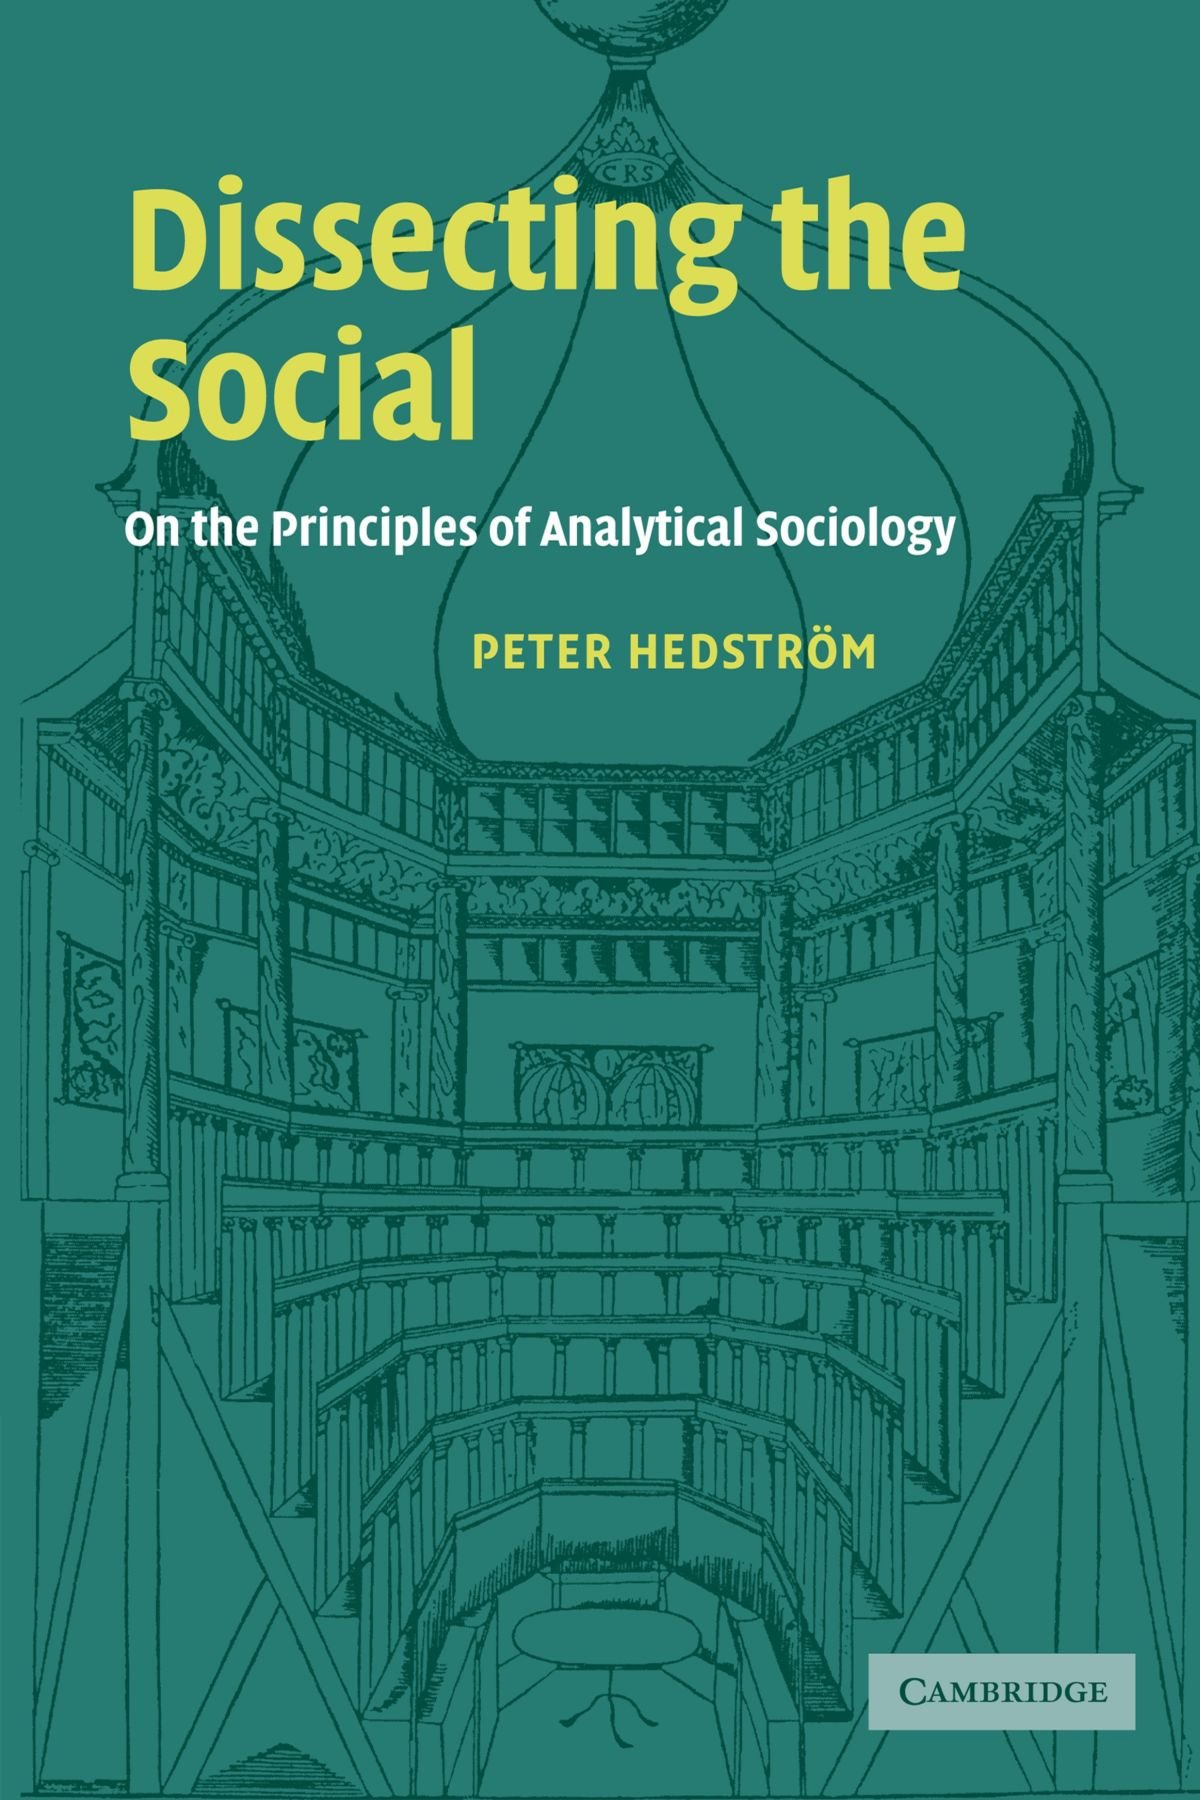
\includegraphics[width=.9\linewidth]{cover.jpg}
\caption{Hedstrom, P. (2005). \emph{Dissecting the Social: On the Principles of Analytical Sociology}. Cambridge: Cambridge University Press. \href{https://doi.org/10.1017/CBO9780511488801}{doi:10.1017/CBO9780511488801}}
\end{figure}

\section*{Overview}
\label{sec:org7f736ec}
\begin{itemize}
\item An explanation of \textbf{Analytical Sociology}.
\item A framework for social theory, with emphasis on mechanisms.
\end{itemize}

\begin{quote}
"[the book discusses] some of the \emph{basic principles of analytical sociology} and soughts to clarify what a \emph{mechanism-based explanatory strategy} looks like" (p. 145).
\end{quote}


\subsection*{Revisiting Coleman's Boat}
\label{sec:orga14f32d}
\begin{figure}[htbp]
\centering
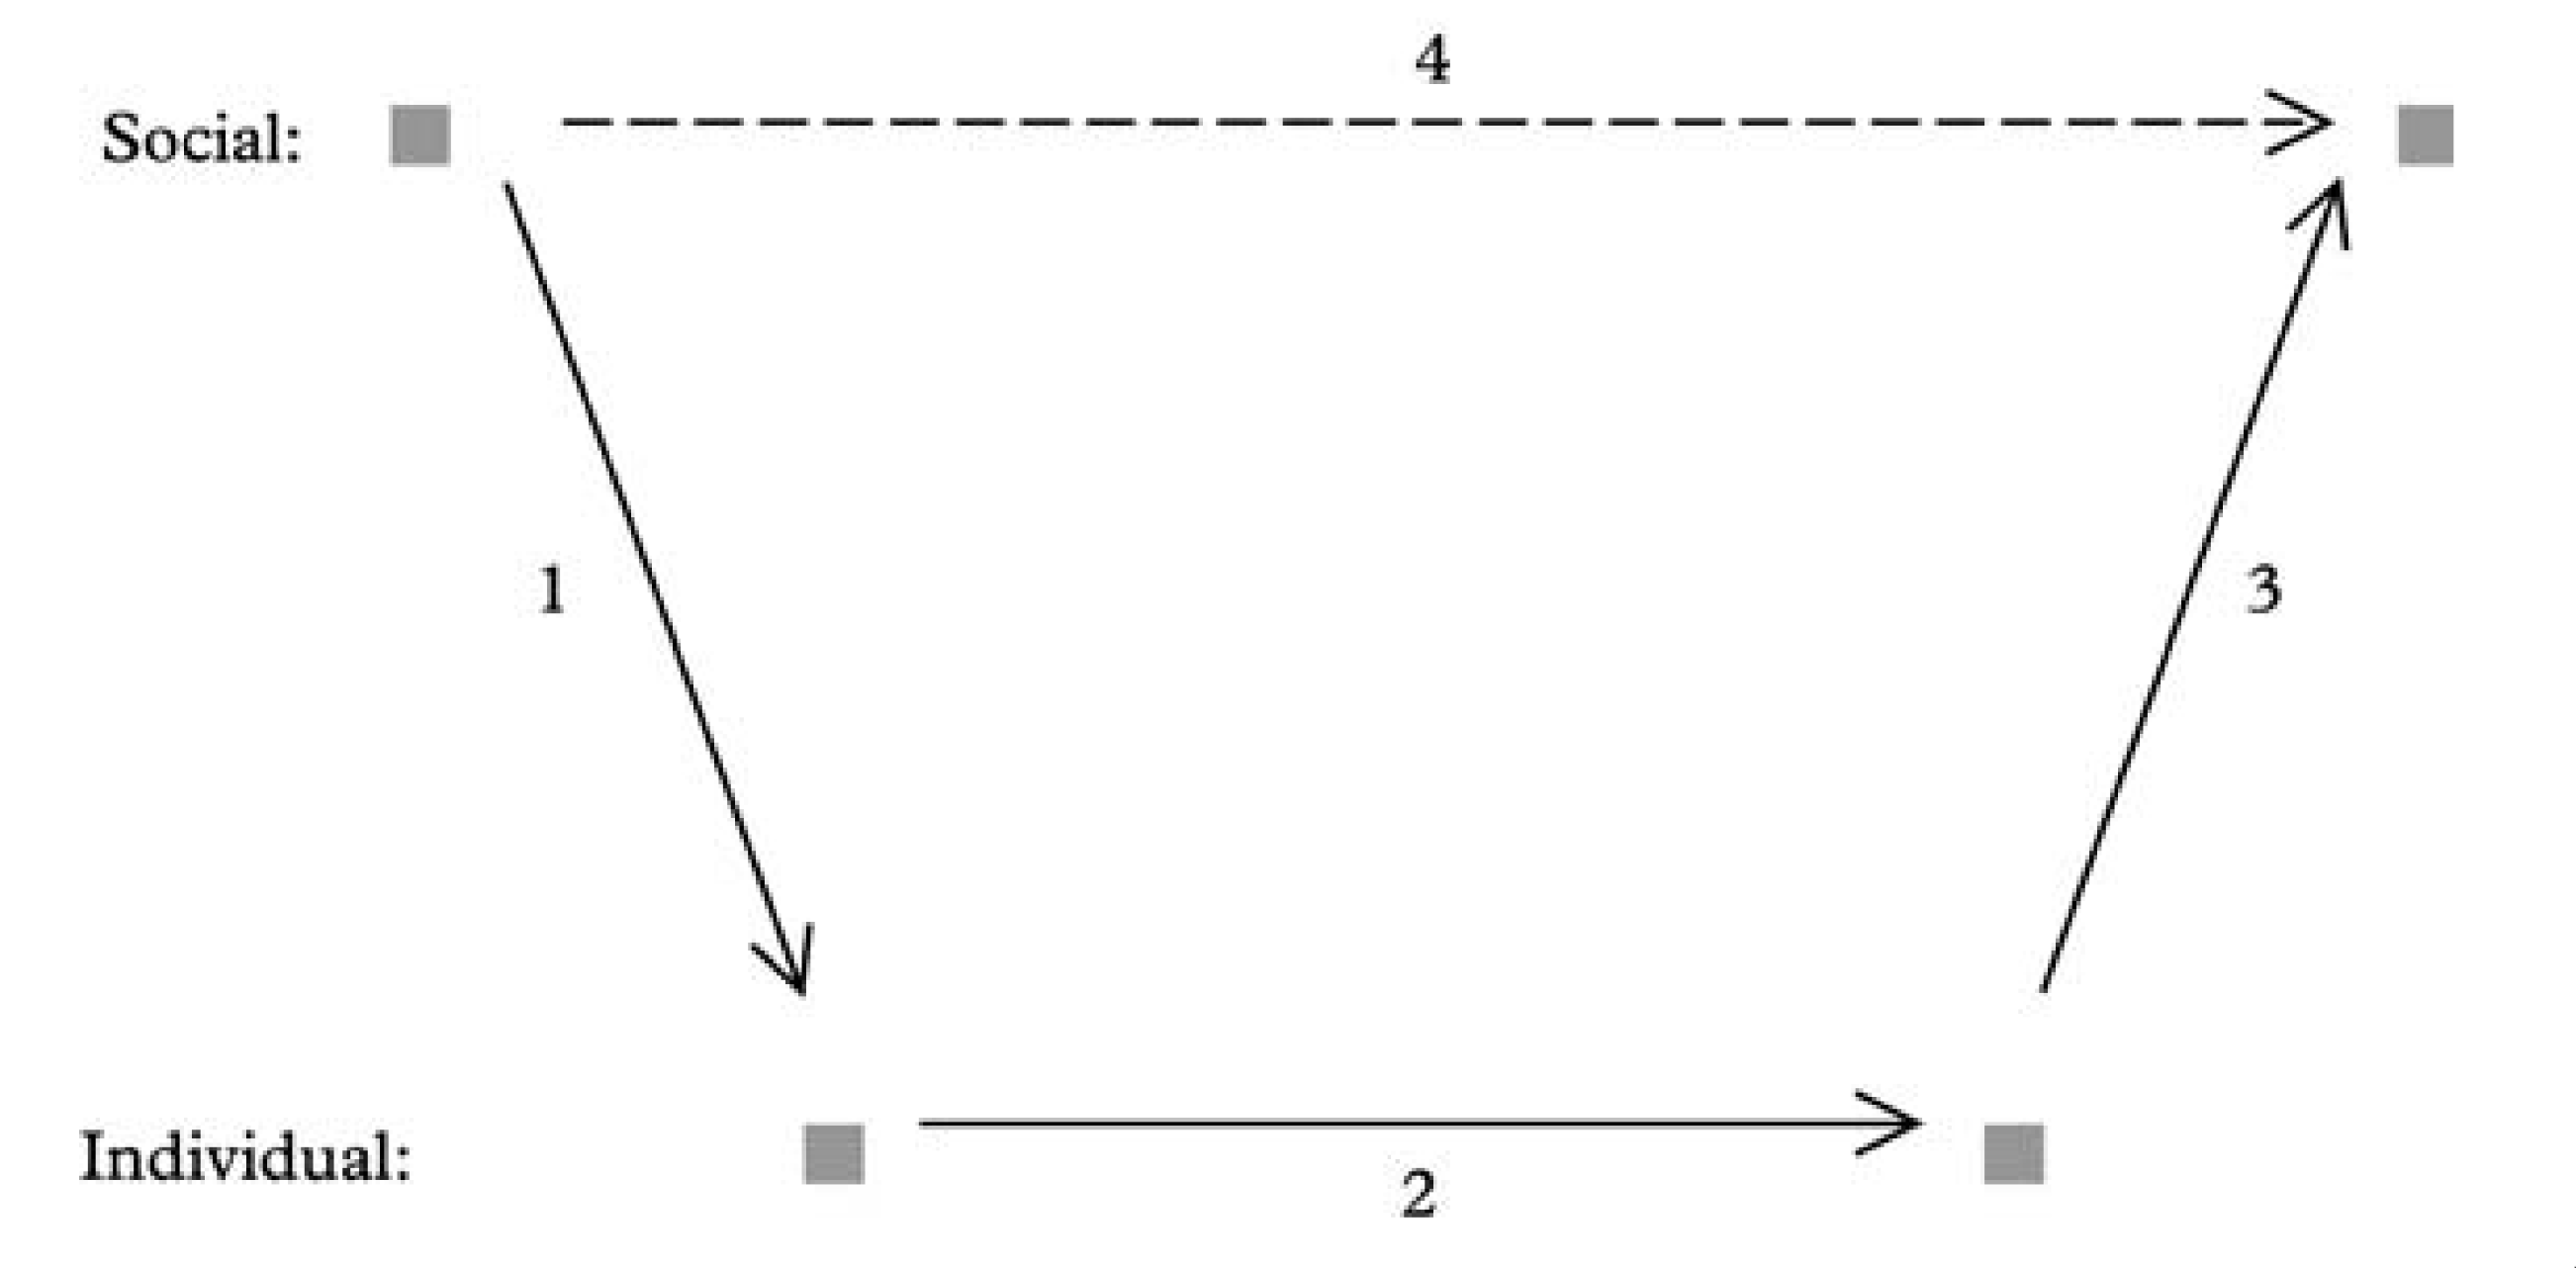
\includegraphics[width=.9\linewidth]{boat.png}
\caption{Coleman's micro-Macro Graph}
\end{figure}

\section*{Table of Contents}
\label{sec:org2dad8e6}
\begin{enumerate}
\item The analytical Tradition in Sociology.
\item Social Mechanism and Explanatory Theory.
\item Action and Interaction.
\item Social Interaction and Social Change.
\item On causal Modelling.
\item Quantitative Research, agent-based modelling and theories of the social.
\item Coda.
\end{enumerate}


\subsection*{Background}
\label{sec:orgb227178}
Three types of explanation.

\begin{enumerate}
\item Covering Law.
\item Statistical.
\item Mechanism based
\end{enumerate}

\subsection*{Foundations}
\label{sec:orgdc4d237}
\begin{figure}[htbp]
\centering
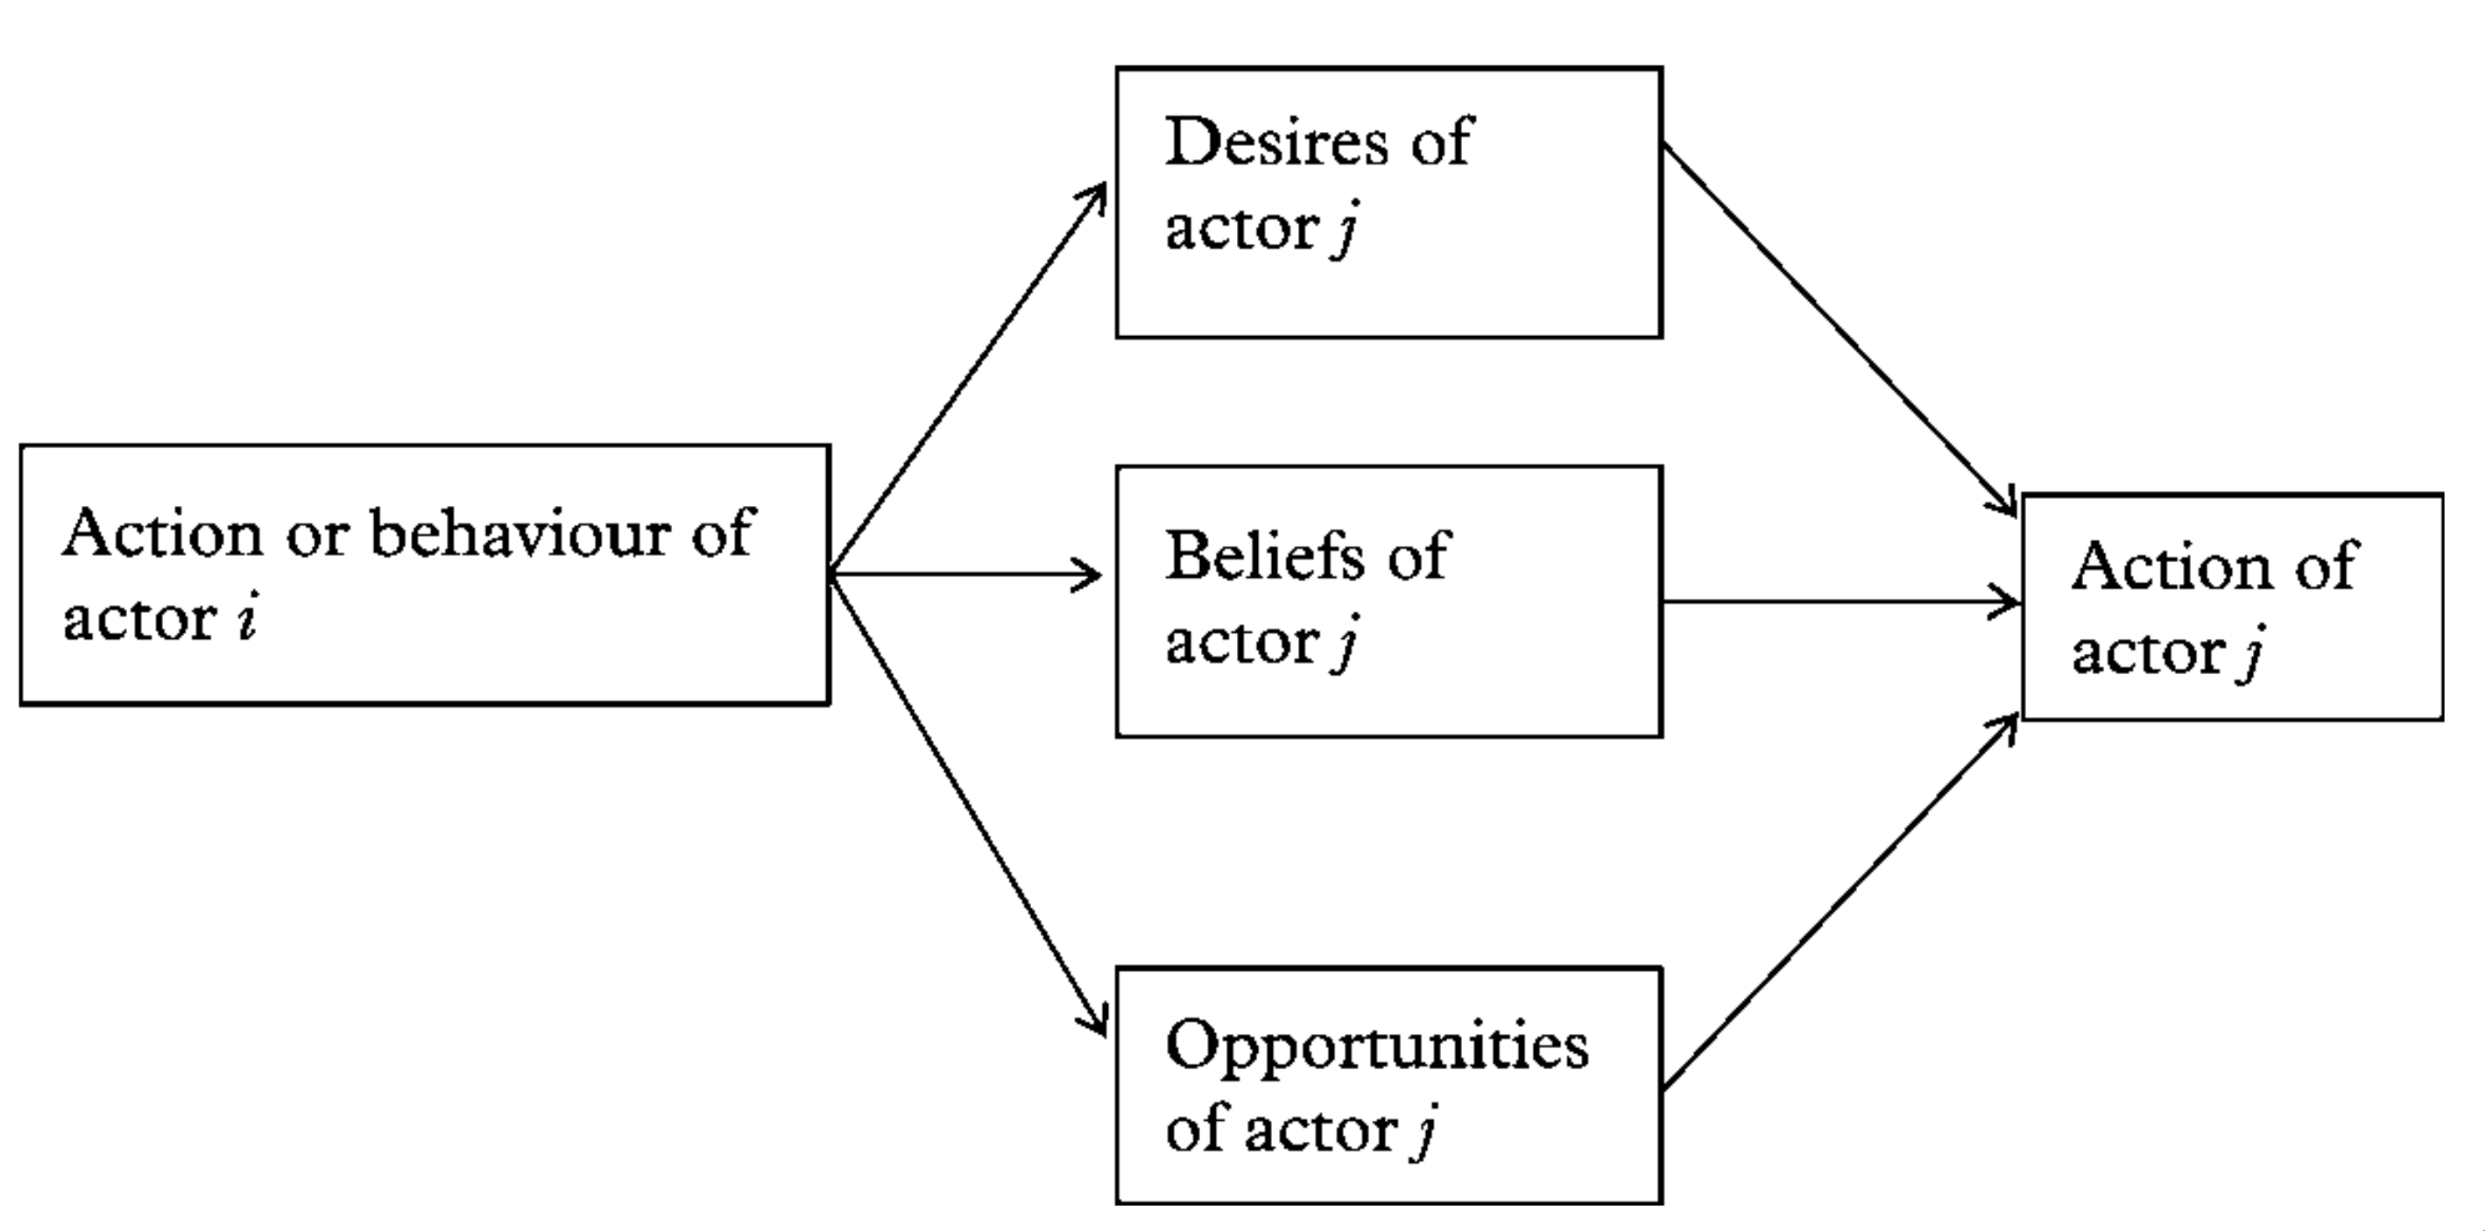
\includegraphics[width=.9\linewidth]{dbo.png}
\caption{D.B.O. Theory}
\end{figure}


\subsection*{Agent Based Models}
\label{sec:org7720a8c}

\begin{figure}[htbp]
\centering
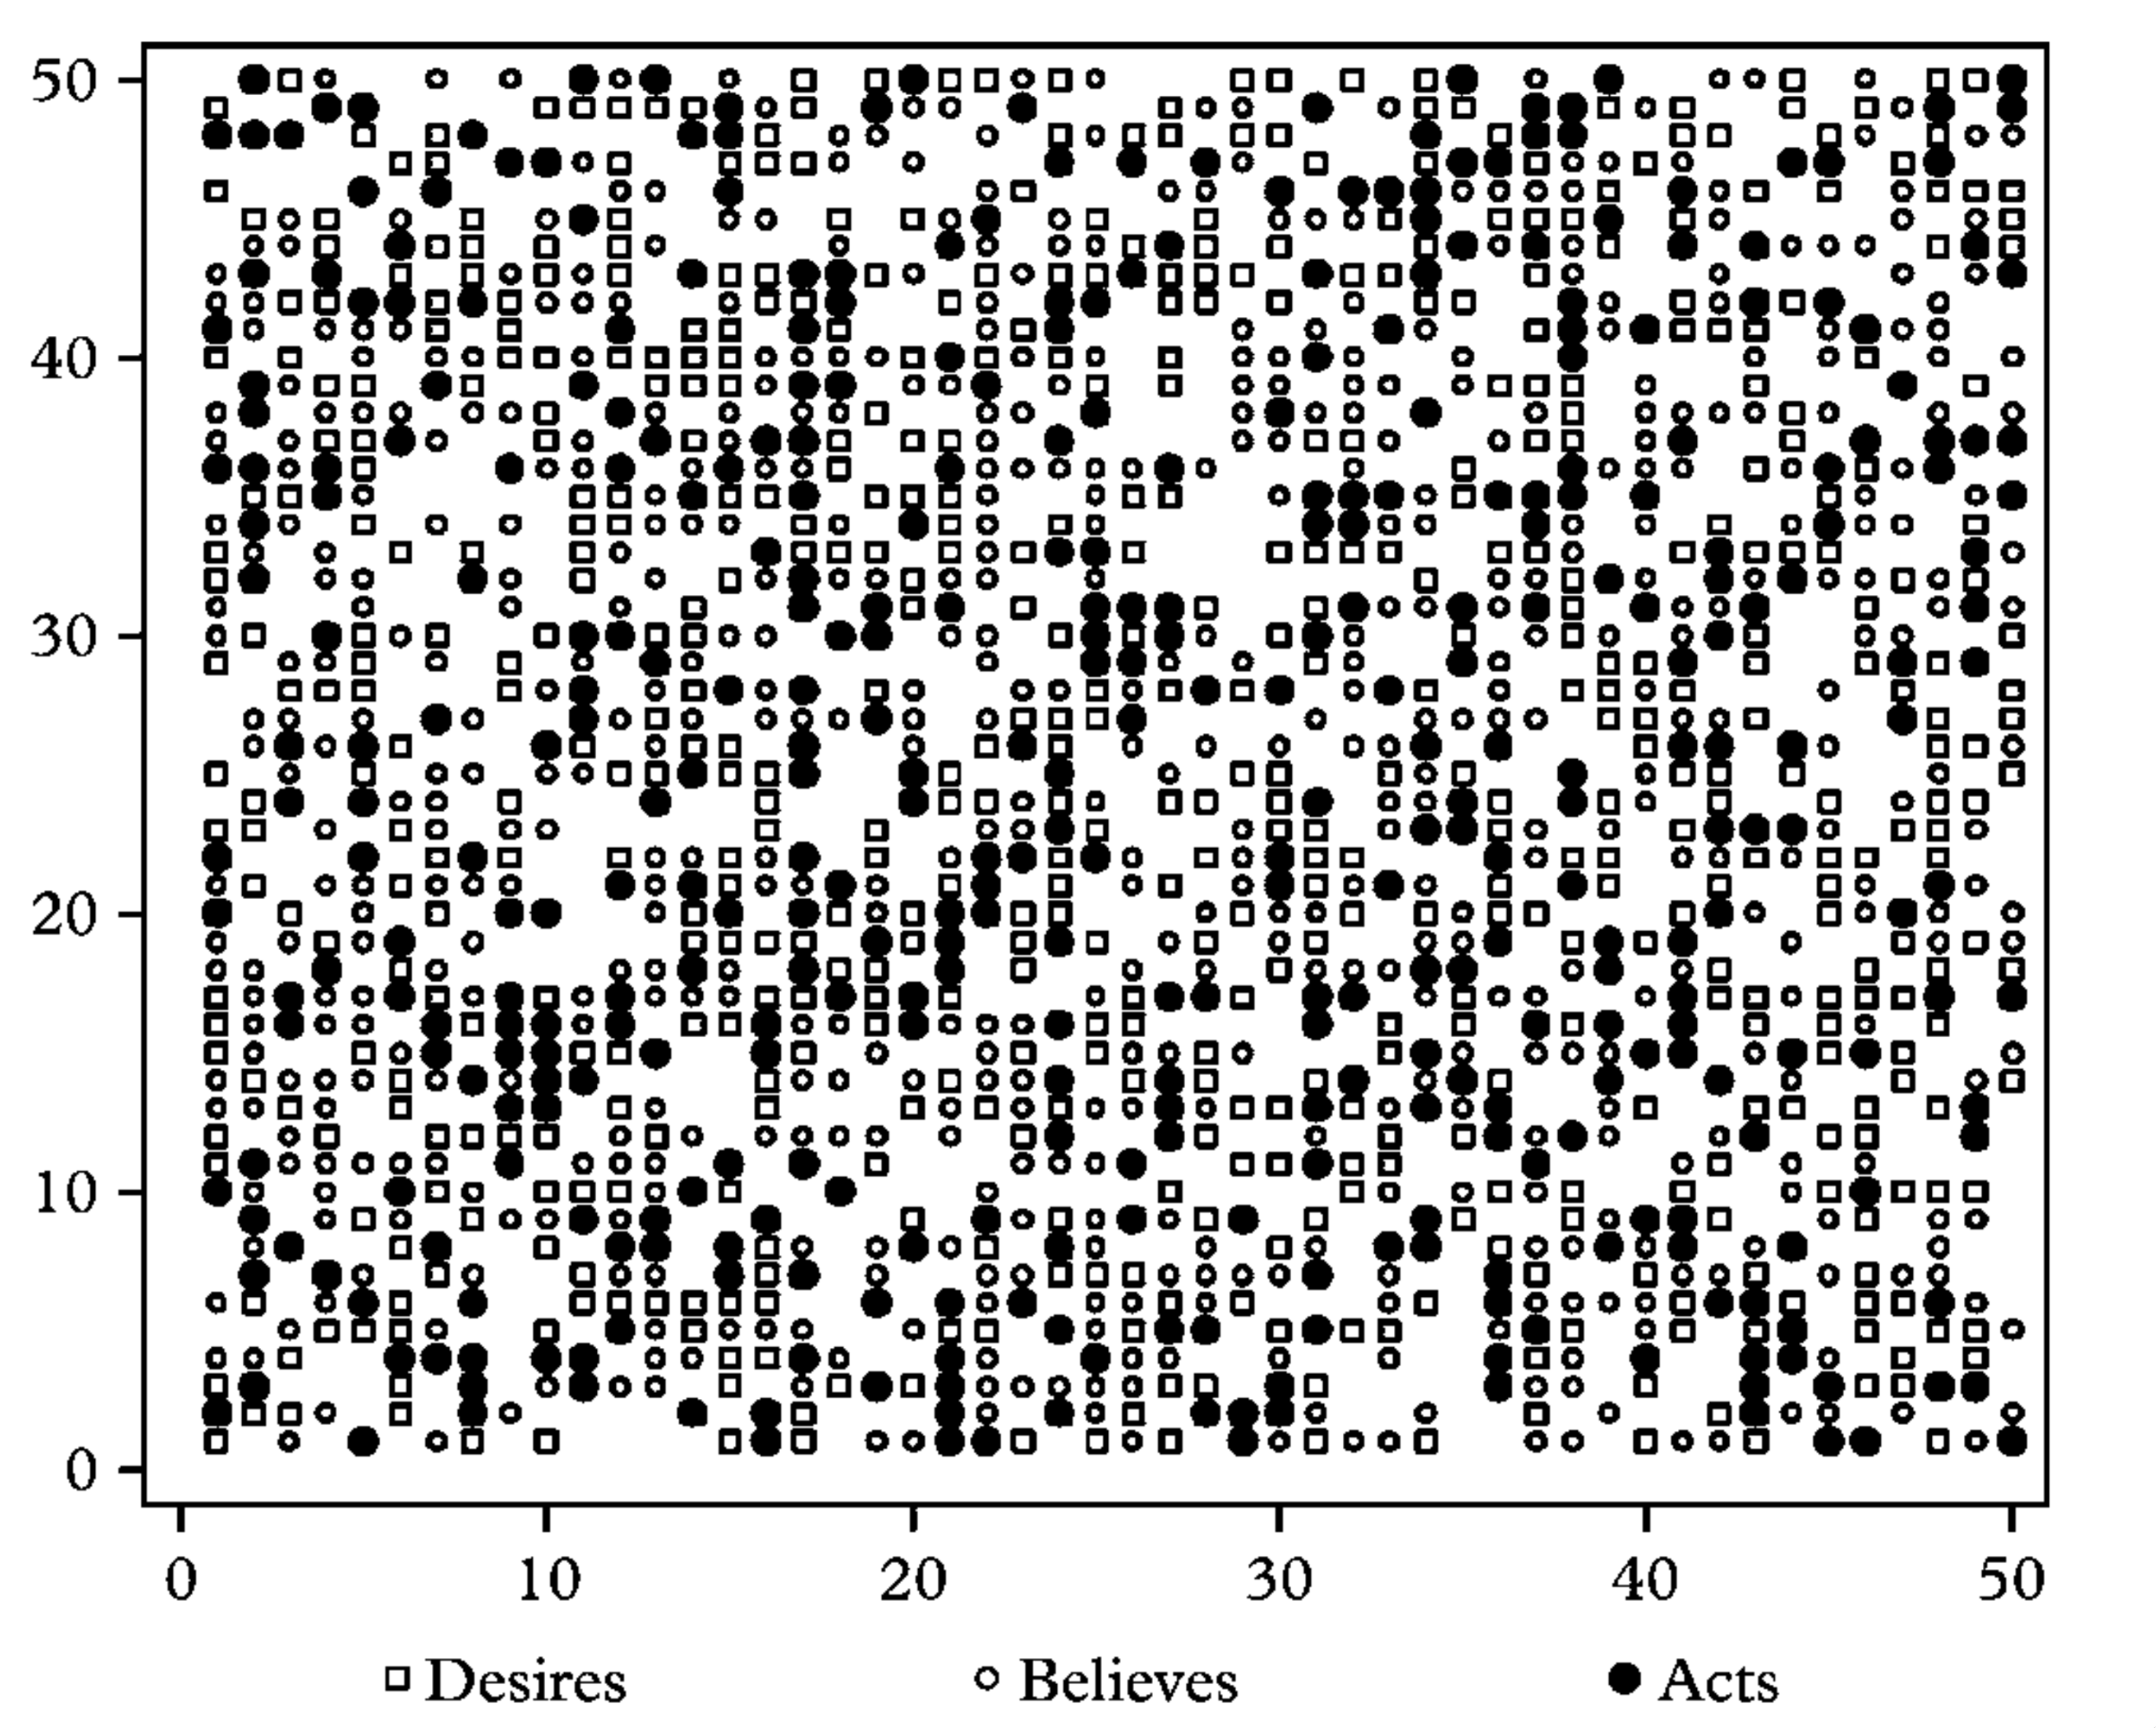
\includegraphics[width=.9\linewidth]{abm.png}
\caption{Initial patterns of beliefs, desires and actions in a population of 2,500 virtual actors.}
\end{figure}


\subsection*{Empirically Calibrated ABM}
\label{sec:org3c859f4}
\begin{figure}[htbp]
\centering
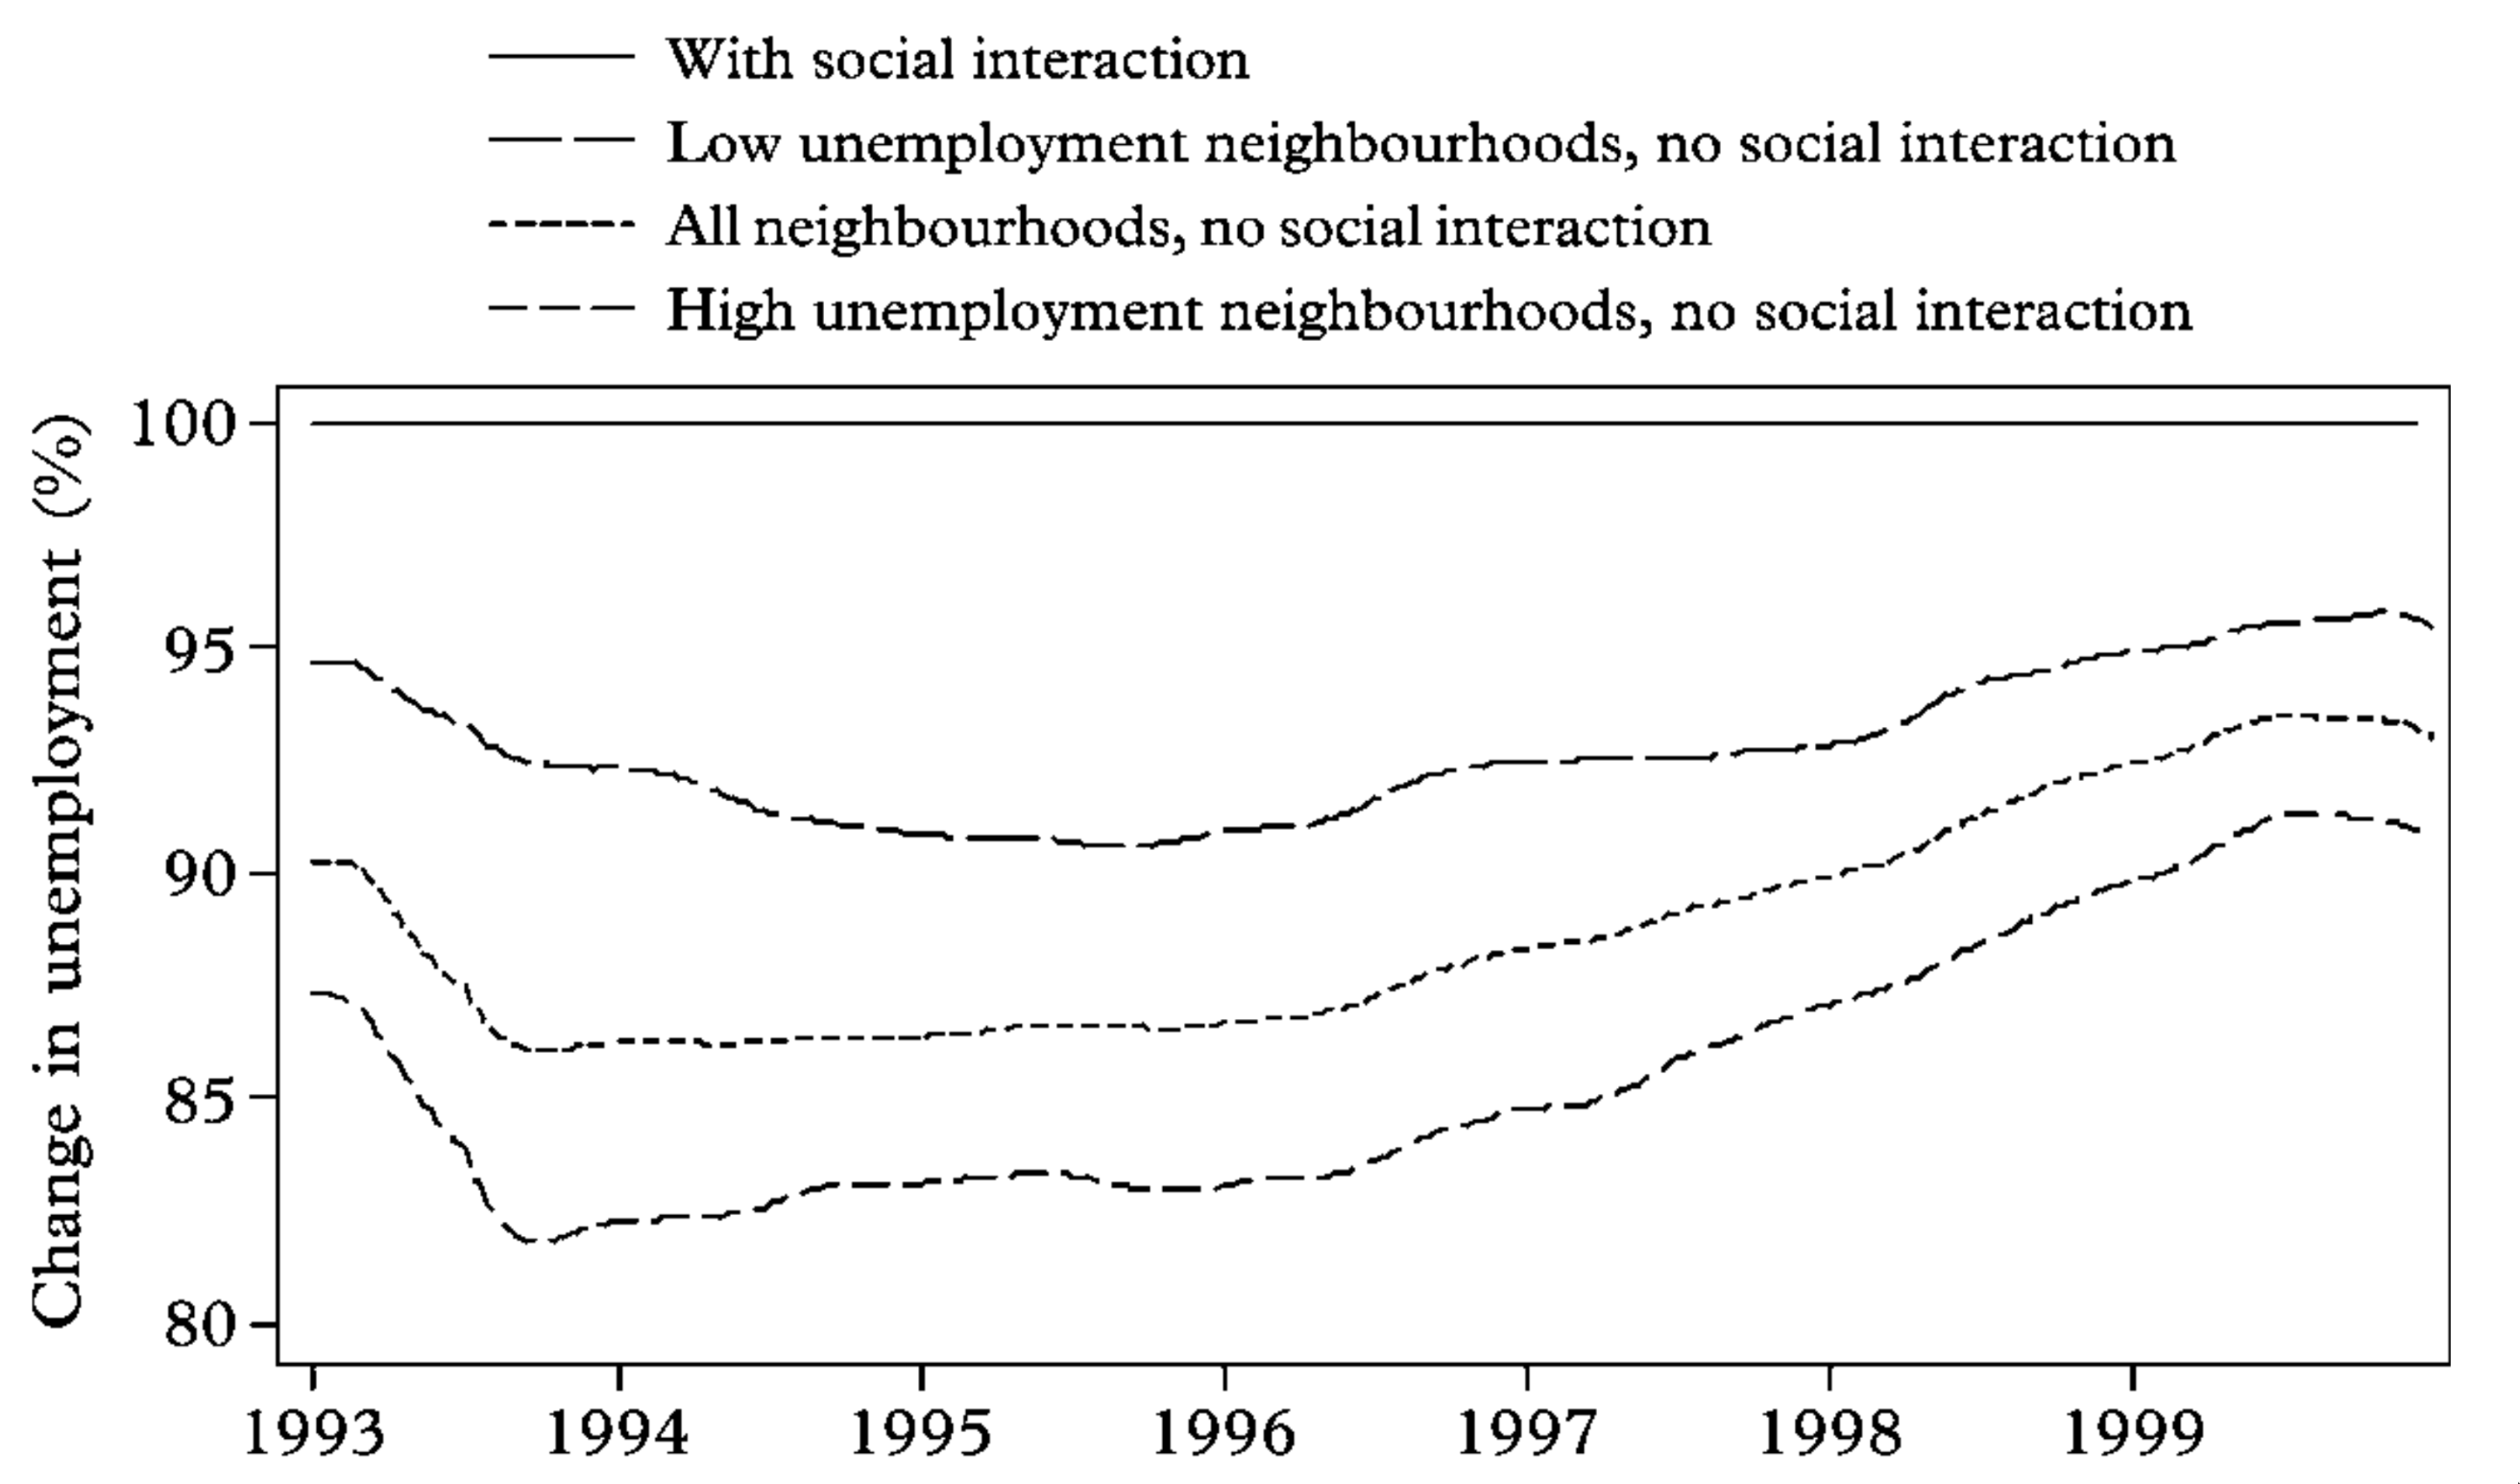
\includegraphics[width=.9\linewidth]{eca.png}
\caption{Unemployment levels and social interactions in low and high unemployment neighbourhoods in the Stockholm metropolitan area.}
\end{figure}




\section*{Opinion on the book}
\label{sec:org100a588}
\end{document}
